\documentclass[tikz]{standalone}
\usepackage[utf8]{inputenc}
\usepackage{amsmath}
\usetikzlibrary{calc}

\def\hash{\mathrm{H}}

\begin{document}

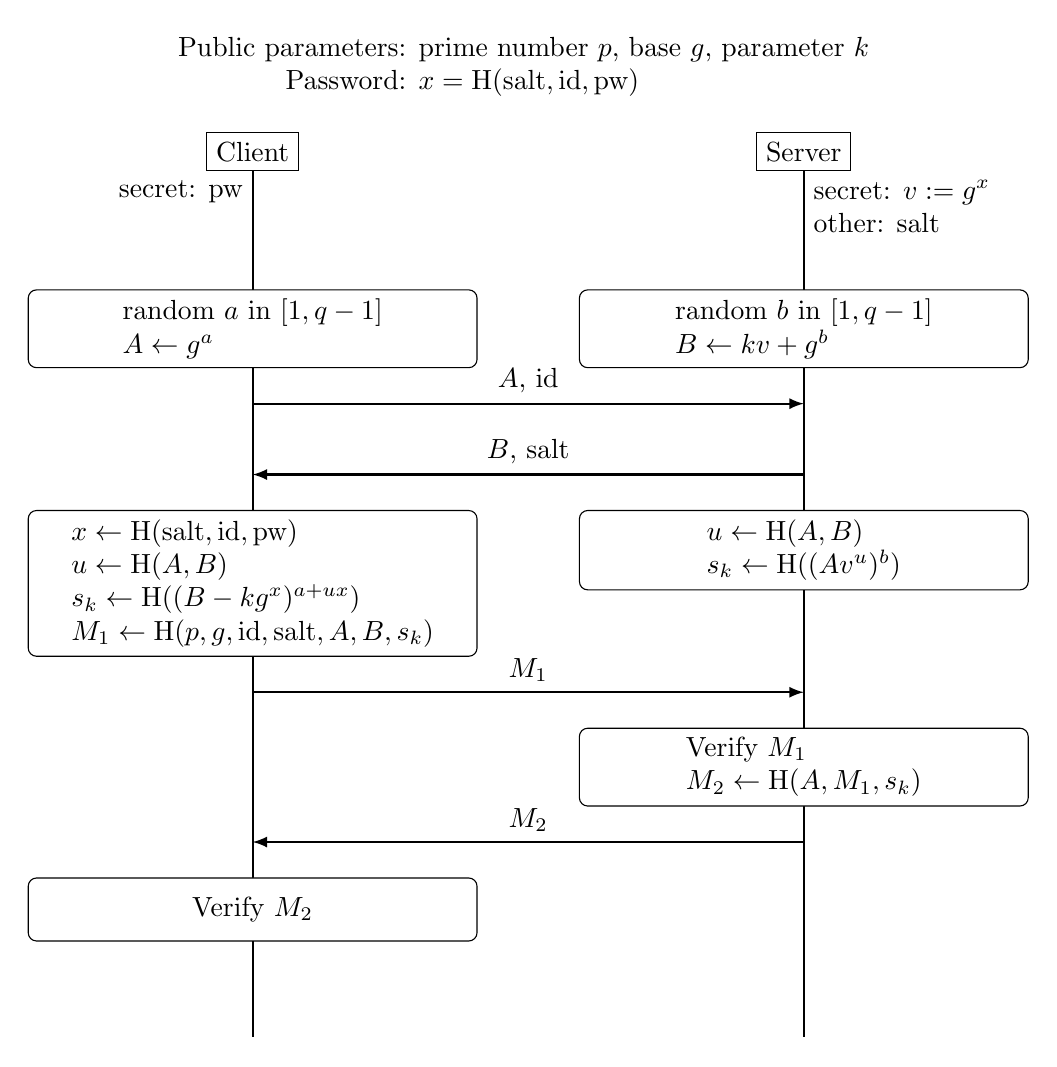
\begin{tikzpicture}[yscale=.9,xscale=.7]
\tikzstyle{box}=[draw,fill=white, rectangle, rounded corners=3pt, align=left, minimum width=5.7cm, minimum height=.8cm]
  
% Public parameters and password
\node[draw=none,fill=none,align=center] (public) at (0,1.2) {%
\vbox{\halign{\hfill# & # \hfill\cr
Public parameters:& prime number $p$, base $g$, parameter $k$\cr
Password:& $x = \hash(\text{salt}, \text{id}, \text{pw})$\cr
}}};
  
% Alice: generate public data
\node[draw] (Alice) at (-5,0) {Client}; 
\draw[thick] (Alice) -- ++(0, -12.5);
\node[below left] at (Alice.south) {secret: pw};
\node[box] (initalice) at ($(Alice) + (0,-2.5)$) {random $a$ in $[1, q-1]$ \\ $A \gets g^a$};

% Bob: generate public data
\node[draw] (Bob) at (5,0) {Server};
\draw[thick] (Bob) -- ++ (0, -12.5);
\node[below right , align=left] at (Bob.south) {secret: $v:= g^x$ \\ other: salt};
\node[box] (initbob) at ($(Bob) + (0,-2.5)$) {random $b$ in $[1, q-1]$ \\ $B \gets kv + g^b$};

% Alice and Bob: generate secret key
\node[box,below] (processalice) at ($(initalice.south) + (0,-2)$) {$x \gets \hash(\text{salt}, \text{id}, \text{pw})$ \\ $u \gets \hash(A, B)$ \\ $s_k \gets \hash((B - kg^x)^{a + ux})$ \\$M_1 \gets \hash(p, g, \text{id}, \text{salt}, A, B, s_k)$};
\node[box,below] (processbob) at ($(initbob.south) + (0, -2)$) {$u \gets \hash(A, B)$ \\ $s_k \gets \hash((Av^u)^b)$};
 
% verification if the session key is the same
\node[box,below] (verifbob) at ($(processalice.south) + (10,-1)$) {Verify $M_1$\\ $M_2 \gets \hash(A, M_1, s_k)$};
\node[box,below] (verifalice) at ($(verifbob.south) + (-10,-1)$) {Verify $M_2$};

% labels on arrows
\draw[-latex,thick] ($(initalice.south) + (0, -.5)$) -- ($(initbob.south) + (0, -.5)$) node [pos=0.5, above] {$A$, id};
\draw[-latex,thick] ($(initbob.south) + (0, -1.5)$) -- ($(initalice.south) + (0, -1.5)$) node [pos=0.5, above] {$B$, salt};

\draw[-latex,thick] ($(processalice.south) + (0, -.5)$) --++ (10, 0) node [pos=0.5, above] {$M_1$};
\draw[-latex,thick] ($(verifbob.south) + (0, -.5)$) --++ (-10,0) node [pos=0.5, above] {$M_2$};

\end{tikzpicture}

\end{document}